\chapter{Nichtstationäre Diffusion}
\label{v:14}

In diesem Versuch betrachten Sie, wie ein Farbstoff in Wasser diffundiert. Dabei messen Sie die momentane Konzentration des Farbstoffes mithilfe eines lichtempfindlichen Widerstandes.

%------------------------------------------------
\section{Stichworte}
%------------------------------------------------

Wheatstone'sche Brückenschaltung; Photowiderstand; Brown'sche Molekularbewegung; stationäre und nichtstationäre Diffusion; Fick'sche Gesetze; Diffusionkoeffizient; Diffusionsgleichung.
%
%------------------------------------------------
\section{Literatur}
%------------------------------------------------

Gehrtsen, Kapitel 5.2.8 und 5.4
%
%------------------------------------------------
\section{Anwendungsbeispiele}
%------------------------------------------------

Diffusion spielt sowohl in der Natur, als auch in zahlreichen technischen Anwendungen eine tragende Rolle.\\
Zum Beispiel geschieht der Gasaustausch zwischen Lungenbläschen und Blut bei der Lungenatmung durch Diffusion, genauso wie der Transport bestimmter Stoffe durch Membranen (teilweise sog. erleichterte Diffusion). \\
Beim Sintern von Werkstoffen spielt die Diffusion eine wichtige Rolle beim Zusammenwachsen der Pulverbestandteile, in der Halbleiterindustrie wird sie benutzt, um Dotierungsstoffe in das Halbleitermaterial einzubringen. In der technischen Chemie spielt Diffusion, gekoppelt mit Konvektion und chemischen Reaktionen eine zentrale Rolle im Reaktor- und Katalysatordesign.

%------------------------------------------------
\section{Theoretischer Hintergrund}
%------------------------------------------------

\subsection{Diffusion in Gasen und Lösungen}

Schichtet man Alkohol vorsichtig über Wasser oder reines Wasser über eine Salzlösung, dann wird die anfangs scharfe Trennfläche allmählich diffuser. Die steile Dichtestufe flacht sich mit der Zeit immer mehr ab. In Lösungen dauert diese Durchmischung Stunden, in Gasen nur Sekunden.\\
Diese Diffusion findet immer dann statt, wenn die Konzentration eines gelösten Stoffes, der Druck eines Gases oder der Partialdruck eines Bestandteiles eines Gasgemisches, allgemein also wenn die Teilchenzahldichte $n$ von Ort zu Ort unterschiedlich ist. Der Vorgang endet erst, wenn die Teilchendichte an allen Punkten des zur Verfügung stehenden Volumens gleich groß ist, falls Teilchen dieses nicht verlassen oder von außen hereinkommen können. Zustande kommt diese Bewegung der Teilchen durch ihre thermische Energie (Brown'sche Bewegung).\\
Der Teilchentransport in der Diffusion wird durch den Gradienten der Teilchenzahldichte, $\mathrm{grad} n$, angetrieben. Die \textit{Teilchenstromdichte} $\vec{j}_n$, ein Vektor, dessen Betrag die Anzahl von Teilchen darstellt, die pro Sekunde durch die Flächeneinheit treten, ist proportional zum Gefälle von $n$:\\

1. Ficksches Gesetz:
\begin{equation}
 \vec{j}_n = -D\,\mathrm{grad}\, n.
 \label{eq:Fick1}
\end{equation}

Der Diffusionstrom fließt immer in die Richtung, in die $n$ am schnellsten abnimmt. $D$ ist der Diffusionskoeffizient, dessen Einheit $\left[D\right] = \mathrm{m^2/s}$ ist.\\

Wenn aus einem Volumen mehr Teilchen ausströmen als hineinfließen, nimmt die Teilchenzahl dort ab:
\begin{equation}
 \dot{n} = -\mathrm{div}\,\vec{j}_n\; .
\end{equation}

Mit Gleichung \ref{eq:Fick1}) erhält man die allgemeine Diffusionsgleichung\\

2. Ficksches Gesetz:
\begin{equation}
 \dot{n} = D\,\mathrm{div}\,\mathrm{grad}\, n = D\,\Delta n\; .
\end{equation}

Diese Art der Diffusion, die durch einen Konzentrationsgradienten getrieben wird, nennt man auch \textit{nichtstationäre Diffusion}. Ihr gegenüber steht die \textit{stationäre Diffusion}, auch Selbstdiffusion genannt, die beschreibt wie sich Teilchen innerhalb derselben Substanz bewegen. Da die Teilchen prinzipiell ununterscheidbar sind, ist die stationäre Diffusion allerdings sehr schwierig zu beobachten.
%------------------------------------------------
\section{Fragen zur Vorbereitung}
%------------------------------------------------

\begin{enumerate}
 %
 %\item Was soll heute im Praktikum gemessen werden? Warum?
 %%
 \item Was ist eine Wheatstone'sche Brückenschaltung? Wie funktioniert sie?
 %
 \item Was ist ein Photowiderstand?
 %
 \item Was versteht man unter Brown'scher Molekularbewegung? Wodurch entsteht sie?
 %
 \item Welcher Effekt wird als Diffusion bezeichnet?
 %
 %\item Was ist stationäre bzw. nichtstationäre Diffusion?
 %
 \item Was ist die Bedeutung der Diffusionskonstanten D (Diffusionsgleichung für stationäre Diffusion) ?
 %
 \item Wie wird ein Photowiderstand zusammen mit einer Wheatstone Brücke zur Messung der Diffusion benutzt ?
%
\end{enumerate}

%------------------------------------------------
\section{Durchführung} 
%------------------------------------------------

\begin{minipage}{0.6\textwidth}
 \begin{enumerate}
  %
  \item Bauen Sie zunächst die Wheatstone'sche Brückenschaltung auf.\\
  
   Der Strom, den das Amperemeter zeigt, hängt bei vorgegebenem Vergleichswiderstand $R_V$ von der Potentiometereinstellung und von dem elektrischen Widerstand des Photowiderstandes $R_P$ ab. Dieser
   Widerstand ist durch die Lichtintensität bestimmt, die auf den Photowiderstand fällt.
  %
 \end{enumerate}
\end{minipage}
%
\begin{minipage}{0.35\textwidth}
 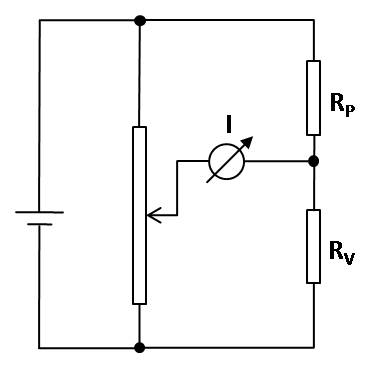
\includegraphics[width=1.00\textwidth]{Abbildungen/Wheatstone14.jpg}
\end{minipage}

\begin{enumerate} \setcounter{enumi}{1}
 %
 \item Stellen Sie den Strahlengang so ein, dass der Beleuchtungsspalt scharf auf den zweiten Spalt abgebildet wird, hinter dem sich der Photowiderstand befindet. Das Amperemeter in der Brückenschaltung zeigt dann den maximalen Strom an. Fixieren Sie den Strahlengang in dieser Konfiguration.
 %
 \item Schieben Sie den Graufilter C016 vor den Photowiderstand und gleichen Sie die Brückenschaltung ab, so dass das Amperemeter keinen Strom mehr anzeigt. Arretieren Sie das Potentiometer in dieser Stellung.
 %
 \item Füllen Sie die Diffusionsküvette zu drei Vierteln mit Wasser und bringen Sie sie anstelle des Graufilters in den Strahlengang, so dass die Wasseroberfläche sich auf gleicher Höhe mit dem Lichtstrahl befindet.
 %
 \item Geben Sie einige Tropfen Farbstofflösung der Anfangskonzentration $C_0$ auf das Wasser und starten Sie zur gleichen Zeit die Stoppuhr ($t=0$).
 %
 \item Verschieben Sie nun die Küvette mittels des Höhentriebes so weit, dass sich die Farbzone mit der Konzentration $C = 1/16\; C_0$ vor dem Spalt befindet.\\
  Diese Farbzone absorbiert Licht genauso stark wie der Graufilter, also zeigt das Amperemeter bei richtiger Einstellung wieder keinen Strom mehr an ($I = 0$). Notieren Sie den Ort $x$ der Farbzone, den man am Höhentrieb ablesen kann.
 %
 \item Wiederholen Sie diese Einstellung zu den Zeiten t = 1, 2, 4, 6, 9, 12, 16, 19, 22, 25, 27, 30, 33, 36 Minuten und notieren Sie jeweils den Ort der Farbzone.
 %
\end{enumerate}

\begin{hint}
\begin{itemize}
 %
 \item Halten sie während der Messung nicht die Stoppuhr an und verstellen Sie nicht das Potentiometer.
 %
 \item Verstellen Sie stets nur den Höhentrieb der Küvette. Bei Manipulation im Strahlengang stellen Sie das Amperemeter auf den Messbereich 'grob'.
 %
 \item Vermeiden Sie größere Erschütterungen des Tisches.
 %
 \item Reinigen und trocknen Sie bitte nach Ende des Versuchs die Küvette gründlich.
 %
\end{itemize}
\end{hint}

%------------------------------------------------
\section{Auswertung} 
%------------------------------------------------
\etodo{Musterauswertung}
\begin{enumerate}
 %
 \item Tragen Sie den Ort $x$ als Funktion von $\sqrt{t}$ graphisch auf. \label{Aufg:1}
 %
 \item Berechnen Sie aus der Steigung der Geraden den Diffusionskoeffizienten $D$ nach:
  \begin{equation}
   D = \frac{x^2}{t}\cdot f\left(\frac{C}{C_0}\right)
  \end{equation}
	
	\noindent
	Bemerkung:\\ 
	\noindent
	$f\left(C/C_0\right) = f\left(1/16\right) = 0,212$ ist ein numerischer Faktor, der die Abhängigkeit des Diffusionskoeffizienten $D$ von der Konzentration der beobachteten Farbzone angibt.
 %
 \item Schätzen Sie den Fehler von $D$ aus den Grenzgeraden der Auftragung aus Aufgabe \ref{Aufg:1}) ab.
 %
\end{enumerate}